\documentclass[twoside]{../zirkelblatt1415}
\usepackage{mathtools}
\usepackage{wrapfig}
\usepackage{float}
\usepackage{booktabs}
\floatstyle{ruled}
\restylefloat{figure}
\restylefloat{table}
\let\raggedsection\centering
\newcommand{\RR}{\mathbb{R}}

\theoremstyle{definition}
\newtheorem{defn}{Definition}[section]
\newtheorem{defn'}{Vorläufge Definition}[section]
\newtheorem{axiom}[defn]{Axiom}
\newtheorem{bsp}[defn]{Beispiel}

\theoremstyle{plain}

\newtheorem{prop}[defn]{Proposition}
\newtheorem{motto}[defn]{Motto}
\newtheorem{wunder}[defn]{Wunder}
\newtheorem{ueberlegung}[defn]{Überlegung}
\newtheorem{lemma}[defn]{Lemma}
\newtheorem{kor}[defn]{Korollar}
\newtheorem{hilfsaussage}[defn]{Hilfsaussage}
\newtheorem{satz}[defn]{Satz}
\newtheorem{thm}[defn]{Theorem}

\theoremstyle{remark}
\newtheorem{bem}[defn]{Bemerkung}
\newtheorem{warnung}[defn]{Warnung}
\newtheorem{aufg}[defn]{Aufgabe}

\definecolor{darkred}{rgb}{0.7,0,0}
\definecolor{shadecolor}{rgb}{.95,.95,.95}

\newenvironment{listing}{
  \renewcommand*\theenumi{\arabic{enumi}}
  \renewcommand{\labelenumi}{\theenumi.}
  \begin{enumerate}\itemsep0em}{\end{enumerate}}

\newcommand{\BB}{\mathrm{BB}}
\newcommand{\defeq}{\vcentcolon=}
\newcommand{\ol}[1]{\overline{#1}}

%\newcommand{\loesung}[1]{\rotatebox{180}{\vbox{#1}}}
\newcommand{\loesung}[1]{#1}

\begin{document}

\maketitleCustom{Klassen 10/11/12}{\textbf{\textsf{%
  Gödels Unvollständigkeitssatz \\
  \normalsize Zirkelzettel vom 7. und 21. November 2014}}}

{\renewcommand{\addvspace}[1]{\vskip0.6em}
\tableofcontents%
}

\section{Einleitung}


\section{Berrys Paradoxon}


\section{Das Halteproblem}

Manche Computerprogramme stoppen nach endlich vielen Rechenschritten
("`halten"'), andere nicht. Etwa hält das Programm "`Lese vom Benutzer eine
Zahl ein, verdopple diese Zahl und gebe das Ergebis aus"', während das Programm
"`Gebe alle natürlichen Zahlen aus"' nicht hält. Im Allgemeinen ist es sehr
schwer, einem Programm anzusehen, ob es hält oder nicht.

\begin{bsp}\label{bsp:unklares-programm1}Die \emph{Goldbachsche Vermutung}
besagt, dass jede gerade Zahl
größer als~3 die Summe zweier Primzahlen ist. Für jede
konkrete gerade Zahl~$n$ größer als~3 kann man das leicht überprüfen, indem man
einfach alle Paare von Primzahlen, die kleiner als~$n$ sind, durchgeht; etwa
sieht man durch Ausprobieren, dass~$14 = 3 + 11$ als Summe zweier Primzahlen
geschrieben werden kann. Noch ist die Vermutung im allgemeinen Fall aber ein
offenes Forschungsproblem. Daher ist nicht klar, ob folgendes Programm hält
oder nicht:
\begin{listing}
\item[1.] Beginne mit~$n \defeq 4$.
\item[2.] Prüfe, ob~$n$ die Summe zweier Primzahlen ist.
\item[3.] Falls ja: Erhöhe~$n$ um Zwei und gehe zurück zu Schritt~2.
\item[4.] Falls nein: Halte.
\end{listing}
Dieses Programm hält genau dann, wenn es ein Gegenbeispiel zur Goldbachschen
Vermutung gibt.
\end{bsp}

\begin{bsp}\label{bsp:unklares-programm2}Eine \emph{Fermatsche Primzahl} ist eine Primzahl der
Form~$2^{(2^n)} + 1$. Die Primzahlen~$3$, $5$, $17$, $257$ und~$65537$ sind von
diesem Typ (für~$n = 0,1,2,3,4$), aber es ist ein offenes Forschungproblem, ob
es weitere Fermatsche Primzahlen gibt. Daher ist von folgendem Programm nicht
klar, ob es hält:
\begin{listing}
\item[1.] Beginne mit~$n \defeq 5$.
\item[2.] Prüfe, ob~$2^{(2^n)}$ eine Primzahl ist.
\item[3.] Falls ja: Halte.
\item[4.] Falls nein: Erhöhe~$n$ um Eins und gehe zurück zu Schritt~2.
\end{listing}
\end{bsp}

Beim \emph{Halteproblem} geht es darum, von einem gegebenen Programm
festzustellen, ob es hält oder nicht. Der britische Logiker, Mathematiker,
Kryptoanalytiker und Informatiker Alan Turing\footnote{Turing leistete während des
Zweiten Weltkriegs entscheidende Beiträge zur Kryptoanalyse der
deutschen Verschlüsselungsmaschine Enigma und ermöglichte so die
Entschlüsselung deutscher Funksprüche. Wegen seiner Homosexualität wurde er
im März~1952 zur chemischen Kastration verurteilt. Er erkrankte an
Depression und beging Suizid.} (*~1912, †~1954) bewies 1937, dass das Halteproblem
\emph{nicht entscheidbar} ist. Genau formuliert bedeutet das:

\begin{thm}Es gibt kein Programm, das bei Eingabe eines beliebigen Programms~$P$ mit einer
korrekten Ausgabe von~"`$P$ hält"' oder~"`$P$ hält nicht"' hält.\end{thm}

Ein hypothetisches solches Programm wird auch \emph{Halteorakel} genannt.
Bemerkenswert an dem Theorem ist, dass es eine absolute Aussage trifft --
Turing behauptet nicht nur, dass \emph{wir} kein solches Halteorakel kennen.
Diese schwächere Behauptung ist auch gar nicht erstaunlich, erfordert doch im
Allgemeinen die Lösung des Halteproblems beliebige offene mathematische
Probleme zu lösen (Beispiele~\ref{bsp:unklares-programm1} und~\ref{bsp:unklares-programm2}).
Vielmehr behauptet Turing, dass ein Halteorakel rein prinzipiell nicht
existieren kann. Auch Außerirdische mit überlegener Technologie oder
transzendente Wesen können kein Halteorakel programmieren.

Programme können durchaus andere Programme simulieren. Das hilft
aber bei der (zum Scheitern verurteilten) Konstruktion eines Halteorakels
nicht: Wir können zwar ein gegebenes Programm~$P$ simulieren und, zum Beispiel,
10.000 Rechenschritte abwarten. Wenn~$P$ bis dahin aber nicht gehalten hat,
wissen wir immer noch nicht, ob~$P$ später halten wird oder nicht.

Einzelne Instanzen des Halteproblems können durchaus algorithmisch
lösbar sein,\footnote{Tatsächlich gibt es sogar für \emph{jedes} Programm~$P$
ein auf~$P$ maßgeschneidertes Orakelprogramm, welches korrekt die Meldung~"`$P$
hält"' oder~"`$P$ hält nicht"' ausgibt. Denn es ist ja klar, dass~$P$ entweder
hält oder nicht hält.  Im ersten Fall ist das triviale Programm, das sich
direkt nach seinem Aufruf mit der Meldung~"`$P$ hält"' sofort wieder beendet,
das gesuchte Halteorakel. Im zweiten Fall ist es das ebenso triviale Programm,
das die Meldung~"`$P$ hält nicht"' ausgibt. Die Situation wirkt vielleicht
etwas wundersam: Eines dieser beiden (trivialen!) Programme ist das gesuchte
Halteorakel, wir können nur im Allgemeinen nicht sagen, welches es ist.}
Turings Resultat sagt nur aus, dass es kein \emph{einzelnes}
Programm gibt, welche \emph{alle} Instanzen des Problems lösen kann -- welches
also bei Eingabe eines \emph{beliebigen} Programms in endlicher Zeit mit der
Meldung~"`hält"' oder~"`hält nicht"' terminiert.

\begin{table}[t]
  \begin{enumerate}
    \item[1.] \texttt{a} \\[-2.0em]
    \item[2.] \texttt{b} \\[-2.0em]
    \item[] $\vdots$ \\[-2.0em]
    \item[26.] \texttt{z} \\[-2.0em]
    \item[27.] \texttt{aa} \\[-2.0em]
    \item[28.] \texttt{ab} \\[-2.0em]
    \item[] $\vdots$ \\[-2.0em]
    \item[41320.] \texttt{bice} \\[-2.0em]
    \item[] $\vdots$
  \end{enumerate}
  \centering
  \caption{\label{tafel:liste-aller-programme}Ein Beispiel, wie die Liste aller
  Programme aussehen könnte, wenn die verwendete Programmiersprache nur die
  Zeichen~\texttt{a} bis~\texttt{z} verwendet.}
\end{table}

\begin{proof}[Beweis des Theorems]
Als Vorbemerkung halten wir fest, dass wir
die Gesamtheit aller Programme in einer unendlichen Liste organisieren können
(Tafel~\ref{tafel:liste-aller-programme}) und darüber hinaus ein Programm~$F$
schreiben können, das bei Eingabe einer natürlichen Zahl~$n$ das~$n$-te
Programm dieser Liste ausgibt.

Angenommen, es gibt ein Halteorakel~$H$.\footnote{Eigentlich müssen wir den
Rest des Beweises in den Konjunktiv setzen, da wir ab dieser Stelle eine Annahme
treffen (mit dem Ziel, einen Widerspruch zu erkennen, um die Falschheit
der Annahme nachzuweisen). Das ist aber umständlich.}
Dann können wir ein Programm~$R$
programmieren, das wie folgt abläuft:
\begin{listing}
\item Lese eine Zahl~$n$ als Eingabe ein.
\item Lasse das Halteorakel ablaufen, um herauszufinden, ob das
Programm~$F(n)$ (also das~$n$-te Programm auf der Liste) bei Eingabe von~$n$
hält oder nicht.
\item Falls es hält: Gehe in eine Endlosschleife.
\item Falls es nicht hält: Halte.
\end{listing}
Das Programm~$R$ zeigt bei Eingabe von~$n$ also genau das entgegengesetzte
Halteverhalten von~$F(n)$.

Wie jedes Programm ist auch~$R$ in der Liste aller
Programme verzeichnet, etwa an~$m$-ter Stelle: Es gilt also~$F(m) = R$.
Wir können uns nun fragen, ob~$R$ bei Eingabe von~$m$ hält oder nicht. Verfolgen
wir den Programmfluss, sehen wir aber, dass beide Fälle zu einem Widerspruch
führen.
\end{proof}

\begin{aufgabeShaded}{Verstanden?}
\vspace{-2em}%
\begin{enumerate}
\item Vollziehe den Beweis des Theorems nach. Könntest du jemand anderem
erklären, welche Widersprüche die Existenz eines Halteorakels nach sich ziehen
würde?
\item Wieso war es für den Beweis wichtig, dass es das Programm~$F$ gibt? Wieso
also war es wichtig, dass wir bei Eingabe einer Zahl~$n$ das~$n$-te Programm
auf der Liste aller Programme berechnen können?
\end{enumerate}
\vspace{-1em}
\end{aufgabeShaded}


\subsection{Turingmaschinen}

\setlength{\wrapoverhang}{1cm}
\setlength{\columnsep}{0.5cm}
\begin{wrapfigure}{r}{0.3\textwidth}
  \vspace{-3em}
  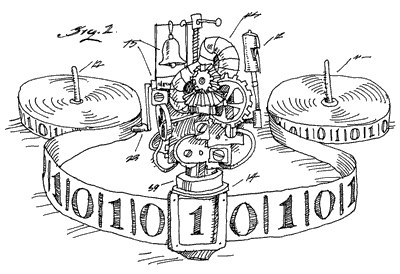
\includegraphics[scale=0.3]{turing-machine}
  \scriptsize
  Eine künstlerische Darstellung einer
  Turing-Maschine.\footnotemark
\end{wrapfigure}
\footnotetext{\url{http://www.worldofcomputing.net/wp-content/uploads/2013/01/turingMachine.gif}}

Was ist eigentlich ein \emph{Programm}? Auf diese Frage sollten wir eine
präzise Antwort haben, wenn wir rigoros Mathematik betreiben möchten. Zur
Vorstellung ist es -- insbesondere, wenn man Programmiererfahrung hat --
hilfreich, sich Programme einer realen Programmiersprache (Haskell, Perl,
Python, \ldots) vorzustellen, welche aber auf \emph{idealisierten Computern}
ablaufen: Computer, die niemals kaputt gehen und über beliebig viel
Arbeitsspeicher verfügen.

Um diese Vorstellung aber zu präzisieren, hat Turing das nach ihm benannte
Konzept der \emph{Turingmaschine} entworfen. Turingmaschinen sind abstrakte
Rechenmaschinen, die sich, weil sie von den vielen Details realer Computer
abstrahieren, für mathematische Untersuchungen besonders gut eignen. Mit
\emph{Programm} meinen wir also eigentlich \emph{Turingmaschine}.

Eine Turingmaschine arbeitet auf einem in beide Richtungen unendlich langem
Band, dessen Zellen die Werte~0 und~1 fassen können.
In jedem Rechenschritt kann die
Turingmaschine den gespeicherten Wert auf dem Band an der aktuellen Position
lesen, einen neuen Wert schreiben und das Band um eine Zelle nach links oder
rechts verschieben. Dabei befolgt sie ein für sie eindeutiges, endliches
Regelwerk.


\subsection{Weitere Übungsaufgaben}

\begin{aufgabeShaded}{Das Halteproblem für halbreale Computerprogramme}
In dieser Aufgabe soll es um Programme gehen, die auf Computern laufen, welche
zwar nie kaputt gehen und auch nicht aufgrund äußerer Einflüsse in ihrem
Verhalten gestört werden (etwa durch kosmische Strahlung), aber trotzdem nur
über endlichen Speicher verfügen. Außerdem sollen sie von der Außenwelt in dem
Sinn isoliert seien, dass sie etwa keine Verbindung zum Internet besitzen.
Kurz und präzise, aber vielleicht weniger anschaulich: Es soll um
Turingmaschinen mit endlichem Band gehen.

Erkläre, wieso das Halteproblem für solche Programme (zumindest in der
Theorie) trivial lösbar ist.

\emph{Tipp:} In wie vielen verschiedenen Zuständen kann sich ein derartiger
Computer befinden?
\end{aufgabeShaded}

\begin{aufgabeShaded}{Der Satz von Rice}
Der \emph{Satz von Rice} ist eine Verschärfung von Turings
Unmöglichkeitstheorem. Er besagt: Für keine nichttriviale extensionale
Programmeigenschaft~$E$ gibt es ein Orakel, das bei Eingabe
eines Programms~$P$ mit einer korrekten Ausgabe von~"`$P$ hat Eigenschaft~$E$"'
oder~"`$P$ hat Eigenschaft~$E$ nicht"' hält.

Dabei meint \emph{nichttrivial}, dass manche Programme die Eigenschaft~$E$
haben und andere nicht. Etwa ist die Eigenschaft~"`$P$ hält oder hält nicht"'
ein Beispiel für eine Eigenschaft, welche \emph{nicht} nichttrivial ist.

\emph{Extensionalität} verlangt, dass sich die Eigenschaft~$E$ nur auf das von
außen sichtbare Verhalten des Programms, nicht aber seine innere Struktur
(seinen Quellcode) bezieht. Etwa sind die Eigenschaften~"`$P$ hält"',
"`$P$ gibt als Ergebnis die Zahl~37 aus"' und "`$P$ gibt eine gerade Zahl als
Ergebnis aus"' extensionale Eigenschaften. Keine extensionalen Eigenschaften
sind~"`$P$ besteht aus weniger als~20 Zeilen Code"' und~"`$P$ tätigt
mindestens~100 Rechenschritte"'.

\begin{enumerate}
\item Überlege, wieso es ganz einfach ist, ein Orakel zu programmieren, dass
die nicht-extensionale Eigenschaft~"`$P$ besteht aus weniger als~20 Zeilen
Code"' prüft.
\item Beweise den Satz von Rice. Du kannst dich dabei am Beweis der
Unentscheidbarkeit des Halteproblems orientieren.
\end{enumerate}
\vspace{-1em}
\end{aufgabeShaded}

\begin{aufgabeShaded}{Die Church--Turing-These}
Informiere dich auf Wikipedia, was es mit der Church--Turing-These auf sich
hat; manche Leute halten sie für eine der größten ungeklärten Fragen der Physik
und Informatik. Hast du eine Meinung dazu?
\end{aufgabeShaded}


\section{Die unberechenbare Fleißiger-Biber-Funktion}

Die \emph{Fleißiger-Biber-Funktion} ist eine Funktion~$\BB : \NN \to \NN$, die
eng mit dem Halteproblem verknüpft ist. Per Definition ist~$\BB(n)$ die größte
Anzahl Rechenschritte, die irgendein haltendes Programm mit
Quelltextlänge~$\leq n$ tätigt.

Anders formuliert: Unter den Programmen mit Länge~$\leq n$ gibt es welche, die
halten, und welche, die nicht halten. Unter denen, die halten, gibt es ein
Programm, dass unter all diesen Programmen am meisten Rechenschritte ausführt,
bevor es schlussendlich hält. Die Anzahl dieser Rechenschritte ist~$\BB(n)$.

Die exakten Werte der Fleißiger-Biber-Funktion hängen von der Wahl der
Programmiersprache ab, denn in verschiedenen Sprachen drückt man sich beim
Programmieren unterschiedlich aus. In der Literatur verwendet man daher die
abstrakten Turingmaschinen als Referenzpunkt.

Die Fleißiger-Biber-Funktion wächst rasant an, viel schneller als exponentiell;
nur sehr wenige Funktionswerte sind bekannt (Tabelle~\ref{tab:bb}). Tatsächlich
wächst sie (asymptotisch) \emph{schneller als jede durch Programme berechenbare
Funktion}. Wie auch bei Turings Unmöglichkeitsresultat liegt der Grund dafür
nicht in menschlichen technologischen Beschränkungen, sondern ist
prinzipieller Natur.

\begin{table}[b]
  \begin{tabular}{@{}lll@{}}
%   \toprule
    $n$ & Anzahl Programme der Länge~$\leq n$ & $\BB(n)$ \\\midrule
    1 & 64 & 1 (1962) \\
    2 & 20736 & 4 (1962) \\
    3 & 16777216 & 6 (1965) \\
    4 & $25{,}6 \cdot 10^9$ & 13 (1972) \\
    5 & $\approx 63{,}4 \cdot 10^{12}$ & $\geq 4098$ (1989) \\
    6 & $\approx 232 \cdot 10^{15}$ & $> 3{,}514 \cdot 10^{18267}$ (2010) \\
%   \bottomrule
  \end{tabular}
  \centering
  \caption{\label{tab:bb}Die bekannten Werte der Fleißiger-Biber-Funktion,
  entnommen aus ihrem
  \href{http://de.wikipedia.org/wiki/Fleißiger_Biber}{Wikipedia-Eintrag}. Mit
  \emph{Programm} ist hier \emph{Turingmaschine} und mit \emph{Länge}
  die Anzahl der Zustände gemeint.}
\end{table}

\begin{thm}Die Fleißiger-Biber-Funktion ist nicht berechenbar, d.\,h. es gibt
kein Programm~$P$, das bei Eingabe einer natürlichen Zahl~$n$ die Zahl~$\BB(n)$
zurückgibt.\end{thm}

\begin{aufgabeShaded}{Unberechenbarkeit der Fleißiger-Biber-Funktion}
\label{aufg:bb}
Beweise das Theorem, indem du folgende Argumentation ausformulierst. Schau dir
erst danach den weiter unten ausgeführten Beweis an.

Wenn es ein Programm gäbe, dass die Fleißiger-Biber-Funktion
berechnen könnte, dann könnte man daraus ein Halteorakel konstruieren (wie geht
das?). Dass es ein solches nicht gibt, wissen wir schon.
\end{aufgabeShaded}

\begin{proof}[Beweis des Theorems]
Angenommen, es gibt ein Programm, dass die Fleißiger-Biber-Funktion
berechnet. Dann können wir mit dessen Hilfe wie folgt ein Halteorakel programmieren:
\begin{listing}
\item Lese ein Programm~$P$ als Eingabe ein.
\item Bestimme mit dem Hilfsprogramm die Zahl~$\BB(n)$, wobei~$n$ die Länge
von~$P$ ist.
\item Lasse~$P$ für~$\BB(n)$ Rechenschritte lang ablaufen.
\item Wenn~$P$ bis dahin gehalten hat: Gib~"`$P$ hält"' aus und beende.
Sonst gib~"`$P$ hält nicht"' aus und beende.
\end{listing}
Dieses Halteorakel arbeitet wirklich korrekt: Denn wenn~$P$ nach~$\BB(n)$
Rechenschritten nicht gehalten hat, wird es niemals halten -- nach Definition
ist ja~$\BB(n)$ die Maximalzahl Rechenschritte, die ein haltendes Programm der
Länge~$\leq n$ ausführen kann, bevor es hält.
\end{proof}


\section{Chaitins Haltewahrscheinlichkeit}

Bevor wir uns der präzisen Formulierung und des Beweises des Gödelschen
Unvollständigkeitssatzes widmen, möchten wir noch einen Abstecher zu
\emph{Chaitins Haltewahrscheinlichkeit}~$\Omega$ machen, einer bestimmte
reellen mit faszinierenden Eigenschaften. In einem Artikel schrieben der
amerikanische Physiker und Informatiker Charles Bennet~(*~1943) und der
berühmte Wissenschaftsjournalist Martin Gardner~(*~1914, †~2010) folgendes über
diese Zahl:\footnote{$\Omega$ embodies an enormous amount of wisdom in a very
small space \ldots{} inasmuch as its first few thousand digits, which could be
written on a small piece of paper, contain the answers to more mathematical
questions than could be written down in the entire universe.

Throughout history mystics and philosophers have sought a compact
key to universal wisdom, a finite formula or text which, when known and
understood, would provide the answer to every question. The use of the Bible,
the Koran and the I Ching for divination and the tradition of the secret
books of Hermes Trismegistus, and the medieval Jewish Cabala exemplify this
belief or hope.

Such sources of universal wisdom are traditionally protected from casual use
by being hard to find, hard to understand when found, and dangerous to use,
tending to answer more questions and deeper ones than the searcher wishes to
ask. The esoteric book is, like God, simple yet undescribable. It is
omniscient, and transforms all who know it.

$\Omega$ is in many senses a cabalistic number. It can be known of, but not
known, through human reason. To know it in detail, one would have to accept
its uncomputable digit sequence on faith, like words of a sacred text.
(C.~Bennett und M.~Gardner, "`The random number~$\Omega$ bids fair to hold
the mysteries of the universe”', Scientific American (1979), Ausgabe 241,
Seiten 20–-34.)}
\begin{quote}
Die Konstante~$\Omega$ verkörpert eine enorme Menge an Wissen auf sehr kleinem Raum.
Die ersten paar Tausend Ziffern, die problemlos auf einem kleinen Stück Papier
Platz finden könnten, enthalten die Antworten auf mehr mathematische Fragen,
als man im ganzen Universum aufschreiben könnte.

Im Laufe der Menschheitsgeschichte strebten Mystiker und Philosophen stets nach einem
kompakten Schlüssel zu universeller Weisheit, einer endlichen Formel
oder einem Text, der, wenn bekannt und verstanden, Antworten auf alle Fragen
liefern würde; man denke nur an die Versuche, der Bibel, dem Koran oder dem I~Ging
Weissagungen zu entlocken [\ldots].

Solche Quellen universeller Weisheit sind herkömmlicherweise vor beiläufigem
Zugriff geschützt: indem sie schwer zu finden, wenn gefunden schwierig zu
verstehen und gefährlich zu benutzen sind, dazu neigend, mehr und
tiefere Fragen zu beantworten als sich der Suchende wünschte. Das esoterische
Buch ist, wie Gott, einfach und dennoch unbeschreibbar. Es ist allwissend, und
verändert alle, die es kennen.

$\Omega$ ist in vielerlei Hinsicht eine kabbalistische Zahl. Dem menschlichen
Verstand ist sie bekannt, aber unkennbar. Um sie im Detail zu erfahren, müsste
man ihre unberechenbare Ziffernfolge als Glaubensgrundsatz einfach hinnehmen,
genau wie die Worte eines heiligen Texts.
\end{quote}

Angesichts dieser Auszeichnung überrascht es vielleicht, dass die Konstante~$\Omega$
durch eine kurze Formel definiert werden kann:
\[ \Omega \defeq \sum_p 2^{-|p|}. \]
Das ist eine Kurzschreibweise, die ausgeschrieben für die unendliche Summe
\[ \Omega := 2^{-|p_1|} + 2^{-|p_2|} + 2^{-|p_3|} + \cdots \]
steht. Dabei ist~$p_1$, $p_2$, $p_3$, $\ldots$ die unendliche Liste aller
\emph{anhaltenden Programme}, und für ein Programm~$p$ steht~"`$|p|$"' für
seine Länge. Die Konstante~$\Omega$ errechnet sich also dadurch, indem man
gedanklich alle anhaltenden Programme durchgeht und
jeweils~$2^{-\text{Programmlänge}}$ addiert. Der Zahlenwert von~$\Omega$ hängt
von der verwendeten Programmiersprache ab; wenn wir eine Definition wünschen,
die nicht von einer solchen willkürlichen Wahl abhängt, können wir
Turingmaschinen verwenden.

Man kann zeigen, dass die unendliche Addition konvergiert, dass durch die
Formel also wirklich genau eine reelle Zahl festgelegt wird, und dass diese
zwischen~$0$ und~$1$ liegt.\footnote{Damit das stimmt, muss man zwei technische
Einschränkungen treffen. Zum einen muss man Programme im Binärsystem notieren,
Programme also durch~0/1-Folgen beschreiben. (Wenn man partout ein Alphabet
aus mehr zwei Zeichen verwenden möchte, muss man in der Definition von~$\Omega$
etwa~$26^{-|p|}$ statt~$2^{-|p|}$ schreiben.) Zum anderen muss die
verwendete Programmiersprache \emph{präfixfrei} sein. Das bedeutet, dass man an
ein syntaktisch korrektes Programm keine weiteren Zeichen anhängen kann, ohne
Syntaxfehler zu verursachen. Beide Einschränkungen spielen im Folgenden aber
kaum eine Rolle.} Die Bezeichnung als \emph{Haltewahrscheinlichkeit} erklärt
sich dadurch, als dass~$\Omega$ gerade die Wahrscheinlichkeit ist, dass ein
willkürzlich gezogenes Programm hält.


\subsection{Unberechenbarkeit und Unkennbarkeit}

Inwiefern sind in~$\Omega$ Antworten auf unzählige mathematische Fragen
enthalten? Darüber gibt die folgende Proposition Auskunft. Um ihre volle
Tragweite würdigen zu können, erinnern wir uns daran, dass wir viele
bedeutende Forschungsprobleme als Fragen der Form "`Hält folgendes Programm?"'
ausdrücken können (Beispiele~\ref{bsp:unklares-programm1}
und~\ref{bsp:unklares-programm2}).

\begin{prop}Kennen wir die ersten~$N$ Nachkommaziffern von~$\Omega$ im
Binärsystem, so können wir das Halteproblem für alle Programme der Länge~$\leq
N$ lösen, also für jedes solche Programm in endlicher Zeit entscheiden, ob es
hält oder nicht.\end{prop}
\begin{proof}Wir machen eine Liste aller Programme der Länge~$\leq N$. Das wird
eine sehr lange, aber endliche Liste. Dann lassen wir all diese Programme
in verzahnter Art und Weise laufen: Wir erlauben jedem Programm, einige
Rechenschritte zu tätigen; danach ist das nächste Programm an der Reihe. Nach
dem letzten Programm auf der Liste kommt wieder das erste an der Reihe.

Im Laufe der Zeit werden immer mehr Programme anhalten. Immer, wenn das
passiert, notieren wir uns die Zahl~$2^{-\text{Länge dieses
Programms}}$. Die Summe dieser Zahlen wird immer weiter anwachsen und sich von
unten der Konstante~$\Omega$ annähern. Sobald diese Summe größer oder gleich
als die als bekannt vorausgesetzte untere Schranke für~$\Omega$ (gegeben durch
die ersten~$N$ Binärziffern) ist, brechen wir alle noch laufenden Programme ab
und ziehen folgende Bilanz:

Alle Programme, die bis zu diesem Zeitpunkt noch nicht angehalten haben, werden
niemals anhalten. Denn diese würden in der Summe die ersten~$N$
Nachkommaziffern beeinflussen. So wissen wir also nun von allen Programmen der
Länge~$\leq N$, ob sie halten oder nicht.
\end{proof}

Die Konstante~$\Omega$ ist also ein Beispiel für eine \emph{unberechenbare
Zahl} -- es kann aus prinzipiellen Gründen kein Programm geben, dass ihre
Nachkommaziffern berechnet. Das unterscheidet sie von anderen wichtigen
Konstanten wie~$\pi$ und~$e$, für die viele Programme zu ihrer Berechnung
bekannt sind.

Es kommt aber noch schlimmer: Die Ziffern von~$\Omega$ sind nicht nur durch
Programme unberechenbar, sie entziehen sich in einem gewissen Sinn auch allen
anderen Arten der Erkenntnis; das ist, was Bennet und Gardner als
\emph{unkennbar} bezeichnet haben. Die genaue Aussage enthält das folgende
Theorem. Leider übersteigt sein Beweis etwas unsere technischen Mittel.

\begin{thm}Zu jedem formalen System gibt es eine Schranke~$N$, sodass für
alle~$n \geq N$ die Aussagen~"`$\Omega$ hat als~$n$-te Nachkommaziffer eine
Null"' und~"`$\Omega$ hat als~$n$-te Nachkommaziffer eine Eins"' in dem System
weder bewiesen noch widerlegt werden können.
\end{thm}

Wenn wir, auf welche Art und Weise auch immer, von den Nachkommaziffern
von~$\Omega$ erfahren würden, könnten wir diese Erkenntnis also nicht beweisen.


\subsection{Informationsgehalt und Zufall}

Die Konstante~$\Omega$ hat eine weitere wundersame Eigenschaft: Ihre
Ziffern sind \emph{Zufallsdaten}. Das ist natürlich nicht wörtlich zu verstehen
-- $\Omega$ ist eine präzise eindeutig definierte Zahl -- aber in einem
gewissen Sinn stimmt es doch. Um das einzusehen, müssen wir uns klarmachen, was
eine \emph{zufällige Ziffernfolge} überhaupt ist. Das ist nicht ganz einfach!
Eine erste Idee, Zufall zu charakterisieren, ist folgende:

\begin{defn'}Eine Ziffernfolge heißt genau dann \emph{zufällig}, wenn in ihr alle
Ziffern im Mittel gleich oft vorkommen.\end{defn'}

Nach dieser Definition würde aber auch die völlig regelmäßige und anschaulich
überhaupt nicht zufällige Ziffernfolge~$01234567890123456789\ldots$ als
zufällig gelten. Etwas besser ist folgende Definition.

\begin{defn'}Eine Ziffernfolge heißt genau dann \emph{zufällig}, wenn in ihre alle
Ziffern, alle Ziffernpaare, alle Zifferntripel und so weiter im Mittel gleich
oft vorkommen.\end{defn'}

Damit gilt~$01234567890123456789\ldots$ nicht mehr als zufällig, denn zum
Beispiel kommt das Ziffernpaar~$00$ überhaupt nicht vor. Allerdings ordnet auch
diese Definition Zahlenfolgen falsch ein, denn die \emph{Champernowne-Folge}
$0123456789101112131415161718192021\ldots$ ist offensichtlich nicht zufällig,
sie erfüllt aber das statistische Kriterium der Definition. Andererseits gibt
es auch Folgen, die anschaulich zufällig sind, das Kriterium aber nicht
erfüllen. Notieren wir etwa die Augenzahlen eines fairen Würfels in einer
Folge, so kommen in dieser Folge gewiss nicht alle Ziffern gleich oft vor --
die Ziffern~$0$, $7$, $8$ und~$9$ kommen überhaupt nicht vor.

Um eine wirklich nützliche Definition von Zufälligkeit zu erhalten, sollten wir
daher Abstand von statistischen Anforderungen nehmen und eher einen
\emph{informationstheoretischen Standpunkt} einnehmen: Lässt sich die
regelmäßige Struktur einer Ziffernfolge in wenigen Worten beschreiben, so
schätzen wir sie als eher unzufällig ein; ist dagegen die einzige Möglichkeit,
die Ziffernfolge zu beschreiben, die, schlichtweg die Ziffern nacheinander
aufzuzählen, so erachten wir sie als zufällig. Im ersten Fall sprechen wir von
einem niedrigen \emph{Informationsgehalt}, im zweiten von einem hohen.

\begin{figure}[b]
  \hfill
  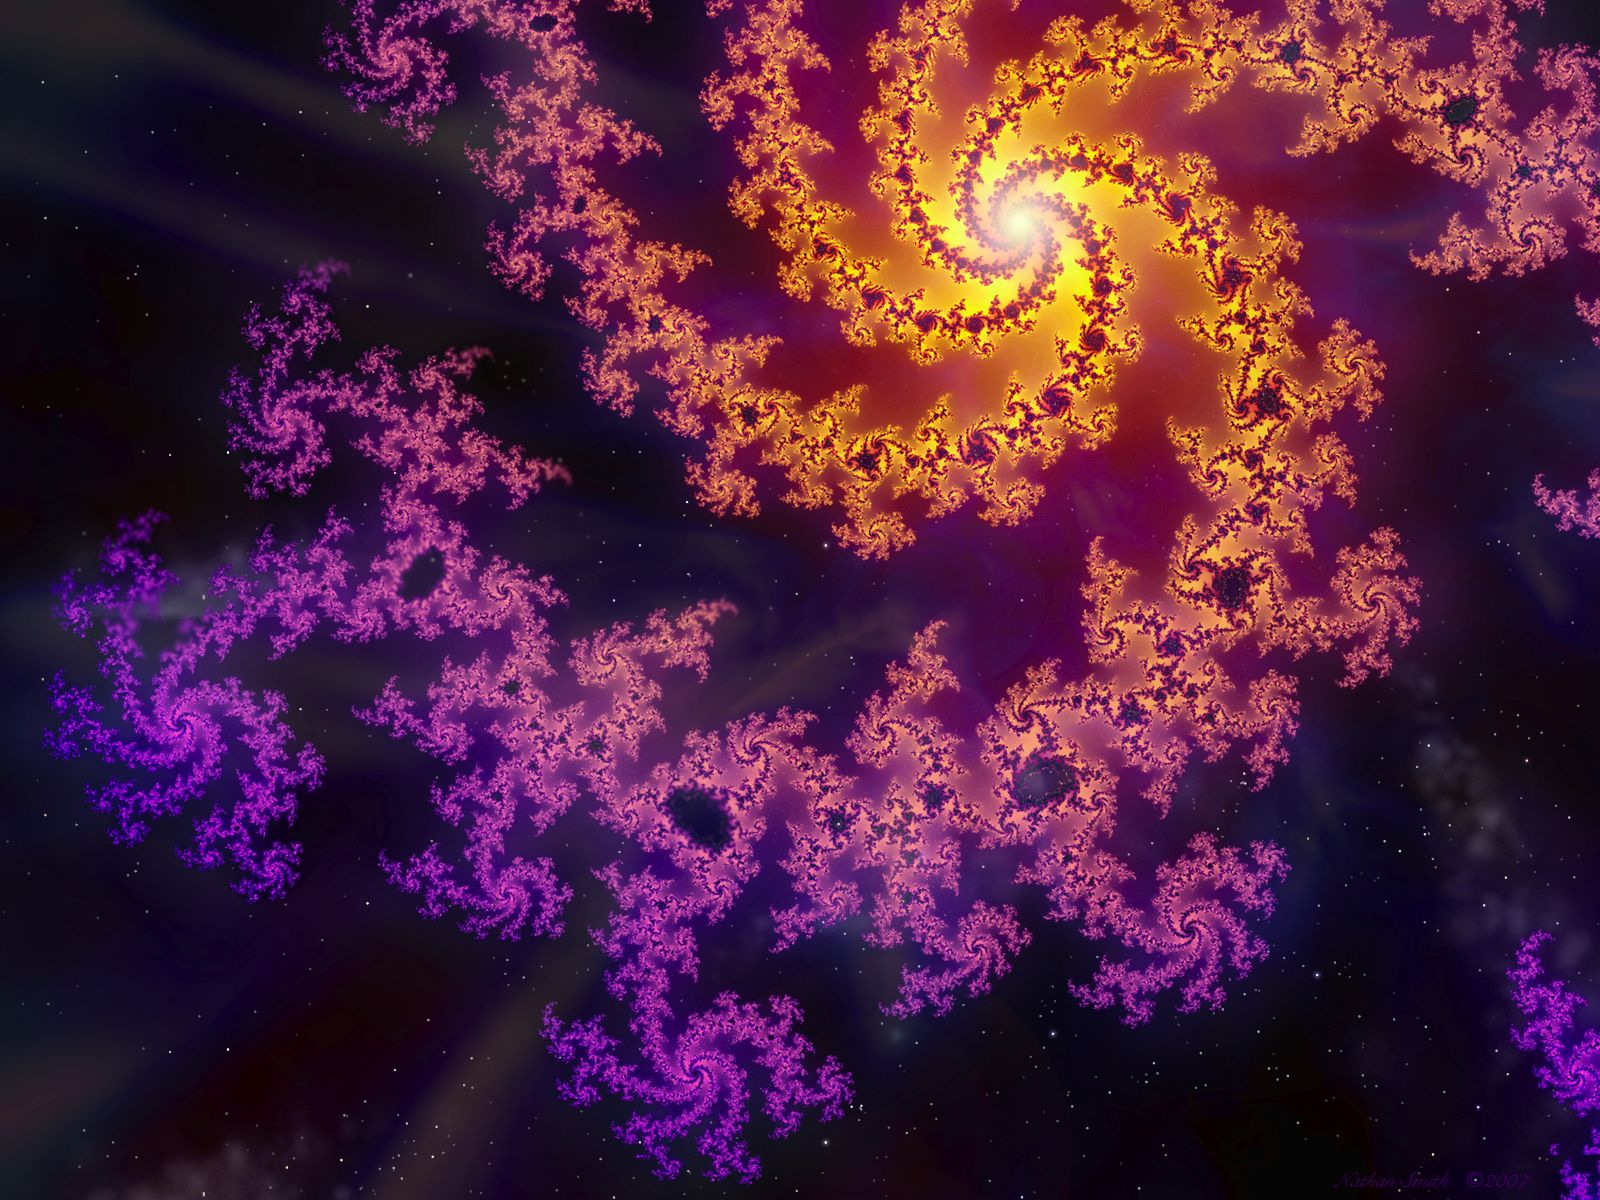
\includegraphics[width=0.4\textwidth]{fraktal1}\hfill
  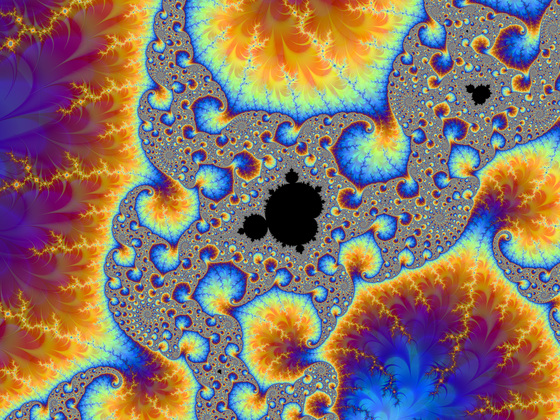
\includegraphics[width=0.4\textwidth]{fraktal2}\hfill
  \centering
  \caption{\label{fig:fraktale}Wer interaktiv in Fraktale dieser Art
  untersuchen möchte, kann sich das freie Programm XaoS herunterladen. \newline
  {\tiny
  \url{http://www.dvice.com/sites/dvice/files/Fractal3.jpg}
  \url{http://upload.wikimedia.org/wikipedia/commons/8/8b/Fractal_KRkr_City1_5600.jpg}}}
\end{figure}

\begin{defn}Der \emph{Informationsgehalt} einer Ziffernfolge ist die Länge des
kürzesten Programms, das diese Ziffernfolge berechnet und ausgibt.\end{defn}

Wir können hier auch an \emph{Beschreibungen durch deutsche Texte} statt an
Programme denken, solange wir nur klare und verständliche Beschreibungen
akzeptieren -- sonst wird, wie bei Berrys Paradoxon, die Definition
widersprüchlich.

\begin{defn}Eine Ziffernfolge heißt genau dann \emph{zufällig}, wenn ihr
Informationsgehalt nicht deutlich kleiner als ihre Länge ist.\end{defn}

Diese Definition lässt sich nicht austricksen. Zum Beispiel erscheint die
aus~325 Ziffern bestehende Folge
\begin{quote}
89793238462643383279502884197169399375105820974944592307816406286 \\
20899862803482534211706798214808651328230664709384460955058223172 \\
53594081284811174502841027019385211055596446229489549303819644288 \\
10975665933446128475648233786783165271201909145648566923460348610 \\
45432664821339360726024914127372458700660631558817488152092096282
\end{quote}

auf den ersten Blick völlig unregelmäßig. Tatsächlich aber handelt es sich
einfach um die Nachkommaziffern von~$\pi$ ab der elften Stelle, ihr
Informationsgehalt ist also viel geringer als~325. Ähnlich verhält es sich mit
den Grafiken in Abbildung~\ref{fig:fraktale}: Wegen ihrer filigranen Struktur könnte man denken, dass
eine präzise Beschreibung dieser Grafiken viel Platz in Anspruch nimmt.
Tatsächlich sind es aber mathematische Fraktale, die schon durch eine kurze
Formel und die Angabe von Koordinaten eindeutig bestimmt sind.

\begin{thm}Die Ziffern von~$\Omega$ sind zufällig.\end{thm}
\begin{proof}[Beweisskizze]Wir haben schon gesehen, dass~$\Omega$ unberechenbar
ist. Ein Programm, dass die ersten~$N$ Nachkommaziffern von~$\Omega$ ausgibt,
kann also die Ziffern nicht auf eine clevere Art und Weise berechnen, sondern
muss sie schon im Quelltext gespeichert haben. Also muss der Quelltext in etwa
selbst schon die Länge~$N$ haben.
\end{proof}


\section{Formale Systeme und Modelle}

Ein \emph{formales System} gibt Axiome und logische Schlussregeln vor.

\begin{bsp}Das formale System \emph{Peano-Arithmetik} (PA) hat als Axiome:
\begin{itemize}
\item Es gibt eine Zahl $\ol{0}$.
\item Jede Zahl~$n$ besitzt einen und nur einen Nachfolger~$S(n)$.
\item Sind~$n$ und~$m$ Zahlen mit gleichem Nachfolger, so sind~$n$ und~$m$
selbst schon gleich.
\item Die Zahl~$\ol{0}$ ist kein Nachfolger einer Zahl.
\item $n + \ol{0} \defeq n$.
\item $n + S(m) \defeq S(n+m)$.
\item $\ol{1} \defeq S(\ol{0})$, $\ol{2} \defeq S(S(\ol{0}))$, $\ol{3} \defeq S(S(S(\ol{0})))$, $\ol{4} \defeq
S(S(S(S(\ol{0}))))$, \ldots
\end{itemize}
Dazu kommen noch einige weitere, insbesondere das wichtige
\emph{Induktionsaxiom}.
\end{bsp}

In dem, was kommt, dürfen wir keinesfalls die \emph{Objektebene} mit der
\emph{Metaebene} verwechseln. Seit Kindesbeinen an kennen wir die gewohnten
natürlichen Zahlen; diese schreiben wir ganz normal, ohne Überstriche:
$0,1,2,\ldots$ Diese natürlichen Zahlen gehören zur Metaebene.

Die Axiome der Peano-Arithmetik sind ein Versuch, unsere Intuition über die
natürlichen Zahlen einzufangen und ihren wesentlichen Kern herauszuarbeiten.
Dabei haben die in den Axiomen verwendeten Symbole~"`$\ol{0}$"', "`$\ol{1}$"'
usw. der Objektebene zunächst \emph{keine inhaltliche Bedeutung}. Insbesondere
beziehen sie sich nicht auf die gewohnten natürlichen Zahlen. Um diesen
Unterschied nicht zu vergessen, notieren wir diese Symbole daher mit einem
Überstrich.

In einem gegebenen formalen System kann man \emph{formale Beweise} führen. Das
sind Beweise, die nur die durch das System vorgegebenen Axiome und
Schlussregeln verwenden.

\begin{bsp}In PA geht ein Beweis der Behauptung~$\ol{2} + \ol{2} = \ol{4}$ wie folgt:
\[
  \ol{2} + \ol{2} = \ol{2} + S(S(\ol{0})) = S(\ol{2} + S(\ol{0})) = S(S(\ol{2} + \ol{0})) = S(S(\ol{2})) = S(S(S(S(\ol{0})))) = \ol{4}.
\]
\end{bsp}

\begin{aufgabeShaded}{Formale Beweise in Peano-Arithmetik}
\begin{enumerate}
\item Vollziehe den formalen Beweis, dass~$\ol{2} + \ol{2} = \ol{4}$ ist, im Detail nach. Welches
Axiom wird in welchem Schritt verwendet?
\item Die Axiome für die Multiplikation lauten
\begin{align*}
  n \cdot \ol{0} &:= \ol{0}, \\
  n \cdot S(m) &:= n \cdot m + n.
\end{align*}
Führe mit diesen Axiomen einen formalen Beweis der Behauptung~$\ol{2} \cdot \ol{2} = \ol{4}$.
\end{enumerate}
\end{aufgabeShaded}

\begin{warnung}Für uns sind die gewohnten natürlichen Zahlen \emph{nicht} durch
die Peano-Axiome definiert. Wir setzen stattdessen voraus, dass wir aus der
Schule und der Erfahrung einen intuitiven Zugang zu natürlichen Zahlen haben.
Wenn man damit nicht einverstanden ist -- etwa, da man das informal erachtet --
muss man die Diskussion in diesem Abschnitt ihrerseits in einem bestimmten formalen
System interpretieren. Irgendwo aber muss man beginnen! Man kommt nicht umhin,
\emph{Metalogik} vorauszusetzen.
\end{warnung}


\section{Gödels Vollständigkeitssatz und sein Unvollständigkeitssatz}

\end{document}

XXX: Das Ende des Beweises über die Nützlichkeit der ersten N Binärziffern von
Omega lässt sehr zu wünschen übrig.


* Unbedingt referenzieren:
  Grenzen der Mathematik: Eine Reise durch die Kerngebiete der mathematischen
  Logik, Dirk W. Hoffmann.

=== Formale Systeme und Modelle

* Ein formales System besteht aus einer Ansammlung von Axiomen und zulässigen
  logischen Schlussregeln.

* Ein Modell für ein formales System ist eine Struktur, in der die Axiome
  und Schlussregeln den Systems gelten.

* Schreibweisen:
  1. S |- phi
  2. M |= phi
  3. S |= phi

* Beispiel: Peano-Arithmetik mit den gewöhnlichen natürlichen Zahlen als
  intendiertes Modell

* Beispiel: wie nichtstandard Modelle der natürlichen Zahlen aussehen.


=== Gödels Sätze

* Vollständigkeitssatz: Wenn S |= phi, dann auch S |- phi.

* Unvollständigkeitssatz: Es gibt phi mit N |= phi, aber nicht PA |- phi.

* Beispiele für Gödel-Sätze:

  * "Dieser Satz hat keinen Beweis."
  * Goodstein-Folgen
  * Aussagen über Ziffern von Omega

* Currys Paradox!
